\documentclass[submission,copyright,creativecommons]{eptcs}

\providecommand{\event}{TFPIE 2022} % Name of the event you are submitting to
% \usepackage{proof}
\usepackage[english]{babel}
\usepackage[utf8]{inputenc}
\usepackage[final]{microtype}
% \usepackage[bottom,multiple]{footmisc}
%
% % paper margins
% \usepackage[margin=.5in]{geometry}
% \pagestyle{plain}
% \usepackage{xspace}
%
% % multiple colums
% \usepackage{multicol}
%
% %Title page settings
% \usepackage[affil-it]{authblk}
%
%
% %% Bibliography
% \usepackage[numbers,sort]{natbib}
% % \usepackage[%
% % backend=bibtex,
% % url=true,
% %style=alphabetic,
% % maxnames=4,
% % minnames=3,
% % maxbibnames=99,
% % giveninits,
% % uniquename=init]{biblatex}
%
% %% Graphics
\usepackage{xcolor}
\usepackage{graphicx}
\usepackage{tikz}
\usepackage{float}
\usepackage{standalone}
 \usetikzlibrary{quotes,angles,calc,arrows.meta,positioning,automata}
\tikzset{initial text={}}
\usepackage{tikz-3dplot}
\usepackage{subcaption}

%% Hyperlinks
\usepackage{url}
\definecolor{pastelblue}{RGB}{0,72,205}
% \usepackage[hidelinks]{hyperref}
\hypersetup{
 colorlinks,
 linktoc=page,
 linkcolor=pastelblue,
 citecolor=pastelblue,
 urlcolor=pastelblue
}
% break urls at dash
\def\UrlBreaks{\do\/\do-}
%
% \usepackage{enumitem}
%
%% Coding
% \usepackage[outputdir=build]{minted}
\usepackage{listings}

\lstdefinelanguage{cyp}{
  keywords={Lemma,goal,Proof,QED,To,show,Case},
  keywordstyle=\color{blue}\bfseries,
  keywords=[2]{data},
  keywordstyle=[2]{\color{purple}\bfseries},
  keywords=[3]{.=.},
  keywordstyle=[3]{\color{red}\bfseries},
  comment=[l]{--},
  commentstyle=\color{purple}\ttfamily,
}

\lstset{
  language=cyp,
  extendedchars=true,
  basicstyle=\ttfamily,
  showstringspaces=false,
  showspaces=false,
  tabsize=2,
  breaklines=true,
  showtabs=false
}
%
% % Math packages
% \usepackage{amsmath}
% \usepackage{mathtools}
% \usepackage{amssymb}
% \usepackage{mathpartir}
% \usepackage{wasysym}
% \usepackage{stmaryrd}
% \usepackage{centernot}
%
% % Proof system
% \usepackage{amsthm}
% %% References
\usepackage[capitalize,sort,compress,noabbrev]{cleveref}
\crefdefaultlabelformat{#2\textup{#1}#3}
\Crefname{thm}{Theorem}{Theorems}
\Crefname{lem}{Lemma}{Lemmas}
\Crefname{prop}{Proposition}{Propositions}
\Crefname{cor}{Corollary}{Corollary}
\Crefname{defn}{Definition}{Definitions}
\Crefname{exmpl}{Example}{Examples}
\Crefname{rmk}{Remark}{Remarks}
\Crefname{propy}{Property}{Properties}
\Crefname{claim}{Claim}{Claim}
\Crefname{assmlisti}{Assumption}{Assumptions}
\Crefname{invarlisti}{Invariant}{Invariants}
%
% \theoremstyle{plain}
% \newtheorem{thm}[equation]{Theorem}
% \newtheorem{lem}[equation]{Lemma}
% \newtheorem{prop}[equation]{Proposition}
% \newtheorem{cor}[equation]{Corollary}
% \theoremstyle{definition}
% \newtheorem{defn}[equation]{Definition}
% \newtheorem{exmpl}[equation]{Example}
% \newtheorem*{rmk}{Remark}

% Custom commands
\newcommand{\jonas}[1]{\textbf{Jonas}: \textcolor{red}{#1}}
\newcommand{\kevin}[1]{\textbf{Kevin}: \textcolor{violet}{#1}}
\newcommand{\lukas}[1]{\textbf{Lukas}: \textcolor{brown}{#1}}
\newcommand{\manuel}[1]{\textbf{Manuel}: \textcolor{green}{#1}}




% Title of document
\title{Engaging, Large-Scale Functional Programming Education in Physical and Virtual Space}

% Author
\author{Kevin Kappelmann \qquad\qquad Jonas Rädle \qquad\qquad Lukas Stevens
\institute{Fakultät für Informatik\\ Technische Universität München, Germany}
\email{\quad kevin.kappelmann@tum.de \quad\qquad raedle@in.tum.de \quad\qquad stevensl@in.tum.de}
}
\def\titlerunning{Engaging Functional Programming Education}
\def\authorrunning{K. Kappelmann, J. Rädle \& L. Stevens}

\begin{document}
%\pagenumbering{gobble}
\maketitle

\begin{abstract}
  World-wide, computer science departments have experienced a dramatic increase in the number of student enrollments.
Moreover, the ongoing COVID-19 pandemic requires institutions to radically replace the traditional way of on-site teaching,
moving interaction from physical to virtual space.
We report on our strategies and experience tackling these issues
as part of a Haskell-based functional programming and verification course,
accommodating \kevin{TODO: find a better word} over TODO students in the course of two semesters.
Among other things,
we fostered engagement with weekly programming competitions
and creative homework projects,
special workshops with industry partners,
and collaborative pair-programming tutorials.
To offer such an extensive programme to hundres of students,
we automated all feedback for programming as well
inductive proof exercises.
We explain and share our tools and exercises such that they can be reused by other educators.

% Notes: what should be in the abstract
% \begin{enumerate}
  % \item rising number of students
  % \item online teaching
  % \item keep quality high
  % \item give good immediate feedback
  % \item keep engagement and interaction high
  % \item do not overwhelm; step by step introduction
  % \item give incentives
  % \item offer space for creativity
% \end{enumerate}

\end{abstract}

%\tableofcontents

%\newpage
%\pagenumbering{arabic}
\section{Introduction}

This paper reports on strategies and solutions employed to
run two iterations of a large-scale functional programming and verification course at the Technical University of Munich (TUM).
While the first iteration (winter semester 2019, 1057 participants)
took place on campus,
the second iteration (winter semester 2020, 1031 participants) was affected by the COVID-19 pandemic and took place in virtual space.
Previous iterations of the course were introduced in~\cite{next_1100};
however, we were facing two novel challenges:

\paragraph{Soaring Enrollments}
The relatively young field of computer science has
become one of the largest study programmes around the globe.
The increase of student enrollments is dramatic
\cite{comp_sci_growth1,comp_sci_growth2}
while employment of new teaching staff often lags behind.
At TUM, the number of new enrollments in computer science more than doubled between 2013 and 2020 from 1110 to 2508 (an increase of 125\%)
, while academic staff only increased from 435 to 529 (21\%) \cite{tum_numbers}.

This drastic increase not only requires more physical resources -- like larger lecture halls and more library spaces --
but also academic staff for supervision.
Given the discrepancy in growth between student enrollments and staff employment,
automation of supervision and feedback mechanisms is inevitable.
Automation, however, should not
negatively affect the quality of the teaching.

\paragraph{Online Teaching}
The ongoing COVID-19 pandemic forced a radical
transition from on-site teaching to online classes.
Lecturers had to rethink the way they present material and interact with students,
teaching assistants the way they assist students in tutorial sessions.
Students, on the other hand, suffer from a lack of social interaction and communication, leading to higher
levels of stress, anxiety, loneliness, and symptoms of depression \cite{students_lockdown1}.

In our experience, the disconnect between students and lecturers, as well as the lack of on-campus interaction between students may also lead to \emph{cramming}:
the practice of showing little participation during the semester
while studying extensively just before the exam.
Cramming tends to result in poor long-term retention and shallow understanding of material.
Indeed, the benefit of spacing learning events apart rather than cramming has been demonstrated in hundreds of experiments \cite{cramming1,cramming2}.

\vspace{\baselineskip}\noindent
Besides these two general challenges,
there is a third -- subject-specific --
challenge we were keen to tackle:

\paragraph{Functional Programming is Practical \kevin{TODO: better paragraph title?}}
Feedback by students and personal experience has shown us that many students
at TUM question the applicability and usefulness
of functional languages beyond
the academia.
They are disappointed by a lack of industrial insight
and real world -- or at least interactive -- applications.
Indeed, some even perceive functional programming as an obstacle;
after all, they already know how to program imperatively.

Good educators do not just teach but inspire:
we have to bring the benefits of functional languages
closer to our students' hearts
by showing real-world applicability and making functional programming fun and engaging.


\vspace{\baselineskip}\noindent
In this paper,
we present our answers to these challenges
and provide tools and exercises for other educators
to make functional programming lectures -- in physical or virtual space -- engaging and scalable.
These resources will be published along the final
version of this article in our central repository\footnote{\url{https://github.com/kappelmann/engaging-large-scale-functional-programming/}}.

\paragraph{Outline}

We begin by describing the general framework and underlying conditions of the course and its syllabus in \cref{sec:course_structure_conditions}.
In \cref{sec:lectures},
we describe the tools and teaching methods that we used during lectures.
\cref{sec:practical_part} describes the
mechanisms and technical setup
we used to create an engaging experience
for the practical part of the course,
including tutorials, homework assignments,
competition systems, and more.
\cref{sec:cyp} introduces
``Check Your Proof'' -- a tool created
by our lab that automatically checks simple inductive proofs for Haskell programs.
\cref{sec:exam} describes how we adapted our exams to the COVID-19 situation and the large number of participants,
and \cref{sec:conclusion} concludes with a summary and aspects to improve in future.


\section{Course Structure and Conditions}\label{sec:course_structure_conditions}

\subsection{Conditions}

The course was mandatory for computer science majors and
an elective for other related degrees such as games engineering or information systems.
All students learnt Java in their first semester and had taken courses on algorithms and data structures,
discrete mathematics, and linear algebra.
The course ran for 14 weeks.

\kevin{TODO: number by Jonas} students registered for
the first iteration\footnote{\url{https://www21.in.tum.de/teaching/fpv/WS19/}} that took place on campus in winter semester 2019 (WS19) and
\kevin{TODO: number by Jonas} for the second iteration\footnote{\url{https://www21.in.tum.de/teaching/fpv/WS20/}} in winter semester 2020 (WS20), taking place in virtual space due to the COVID19 pandemic.

Both iterations were organised by the lecturer, Tobias Nipkow, and the authors of this paper.
The first designed the course, created the slides\footnote{\url{https://www21.in.tum.de/teaching/fpv/WS20/assets/slides.pdf}}, and gave the lectures.
The others took care of the practical and organisational part of the course.
All gained valuable experience in running an online course on the theory of computation for \kevin{TODO: number Jonas}
students in summer semester 2020.
Finally, Manuel Eberl had the honour of being the \emph{Masters of Competition Senior} and assisting us with the weekly programming competition (see \kevin{TODO: reference}).

Needless to say,
running tutorials for more than 1100
students each semester by our own is impossible.
We were further assisted by
\kevin{TODO: Jonas numbers} student assistants in WS19 and
\kevin{TODO: Jonas numbers} student assistants in WS20.
In WS19, their primary job was to run the tutorials and provide feedback for homework submissions (e.g.\ code style improvements).
However, it became clear to us
that the feedback so provided was not effective
and that their time is better used by creating engaging exercises in WS20 (see \kevin{TODO: reference}).

% As written before, the rapid growth in number of students (225\% in seven years)
% far exceeds the growth in academic staff (121\%).



\subsection{Syllabus}

The course deals with the basics of functional programming and the verification of functional programs.
Most parts of the course could be done using any functional language.
We chose Haskell because of its simple syntax, large user community, and good testing facilities (in particular QuickCheck).
The syllabus of the course stayed close to the one presented in~\cite{next_1100}.
Notable changes include the omission of the parser case study -- parsing problems were instead introduced in homework exercises -- and the rigorous introduction of computation induction and type inference.

Concepts are introduced in self-contained small steps.
Characteristic features of functional programming languages such as
higher-order functions and algebraic data types are
only introduced midway through the course.
This makes the design of interesting practical tasks harder
but ensures that students are not overwhelmed by the diversity
of new principles that are not part of introductory imperative programming courses.
In general, the course progresses from ideas close to what is known from imperative languages (e.g.\ boolean conditions, recursion on numbers, auxiliary functions, etc.)
to simple applications of new concepts (e.g.\ recursion and induction on lists)
to generalised new concepts (e.g.\ algebraic data types and structural induction).




\section{Lectures}\label{sec:lectures}

Concepts are introduced in self-contained small steps, one by one.
Characteristic features of functional programming languages such as
higher-order functions and algebraic data types are
only introduced midway through the course.
This makes the design of interesting practical tasks harder
but ensures that students are not overwhelmed by the diversity
of new principles that are not part of introductory imperative programming courses.

Each self-contained topic comes with small case studies and examples.
The latter are accompanied by suitable QuickCheck tests
and inductive correctness proofs when appropriate (more details in \cref{sec:cyp}).

The lecturer presents topics using a mix of
slide presentations,
live coding, and whiteboard proofs.
Students can interact and ask questions at any time.
During the online semester,
lectures were livestreamed and
engagement made possible by means of a live Q\&A stream.
The stream was moderated by a PhD student
sitting in the same room as the lecturer.
Questions could be answered by students as well as the moderator.
The moderator approved and answered individual and simple questions directly while putting forward those questions to the lecturer
that were of a more general nature.
Those questions were not put forward due to a lack of understanding of the moderator
but to increase engagement between students and the lecturer,
a point of critic often raised by students in our department.

We can report that this moderated format increased engagement when compared to the physical format of the first semester:
students were less reluctant to submit questions for
1) they had the chance to ask question anonymously,
2) they were not afraid to ``interrupt'' the lecture, and
3) they were able to ask new kind of questions.
Examples of the third include discussion of alternative solutions by students,
organisational questions,
and slightly off-topic discussions that nevertheless increase engagement and curiousity.

Following the livestream,
the recordings were also uploaded for asynchronous consumption.


\section{Practical Part}\label{sec:practical_part}

\subsection{Engagement Mechanisms}

\kevin{TODO: probably move to intro}
One main concern of educators around the globe is cramming:
the practice of studying extensively just before the exam while
showing little participation during the semester.
Cramming tends to result in poor long-term retention and shallow understanding
of material.
Indeed, the benefit of spacing learning events apart rather than cramming has been demonstrated in hundreds of experiments \citep{cramming1,cramming2}.

To prevent cramming,
we used a variety of engagement mechanisms and incentives as the course progresses.
Good engagement mechanisms not only keep students busy
but genuinely make the course more fun.
Participation should originate from curiosity and enjoyment rather than pressure.
In the best case, students might even study beyond the material presented
if given the possibility.

\paragraph{Grade Bonus}
Grade bonus: re-introduced after low engagement in last iteration

\paragraph{Instand Feedback}
TODO

\paragraph{Wettbewerb and Awards}
TODO

\paragraph{Social Interactions}
Pair-Programming, FPV\&Chill, Contest

\paragraph{Workshops with Industry Partners}
TODO


\subsection{Technical Setup and Automated Assessment}\label{sec:tech_setup_test}

\paragraph{Automated Assessment}
In WS19, we used an improved version of
the testing infrastructure introduced in \citep{next_1100}.
However, this system was not able to manage online exams and mark freeform submissions.
We thus switched to use a newly written open-source
tool developed at TUM called ArTEMiS \citep{artemis}.
ArTEMis is a highly scalable, automated assessment management system.
It already offered support for a few imperative programming languages
and we added support for Haskell\footnote{It now also supports OCaml}.
As ArTEMis takes care of anything from load-balancing to
automated testing and
offers a special exam mode and good support for freeform submissions,
the only thing we were left to do is writing the actual test code.
More details about ArTEMis and our test setup follow
in the extended version of this article.

\paragraph{Online Tutorials}
% Due to the COVID19 pandemic,
% we realised that online tutorials will not b


% Previous iterations of the course did
% not make any recommendations about the editor to be used for
% the practical part of the course.
% the retake exam of the WS19 iteration had to take place online.
% \footnote{\url{https://www21.in.tum.de/teaching/fpv/WS20/installation.html}}


\subsection{Selected Exercises and Tools}\label{sec:selected_exercises}


\begin{figure*}[t!]

\centering
\begin{subfigure}[t]{0.3\textwidth}
  \centering
  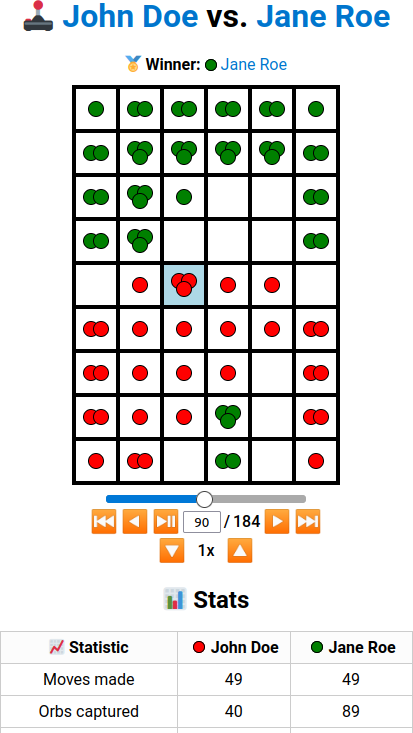
\includegraphics[width=\linewidth]{img/chainreaction}
  \caption{Game tournaments}
  \label{fig:chainreaction}
\end{subfigure}%
~
\begin{subfigure}[t]{0.3\textwidth}
  \centering
  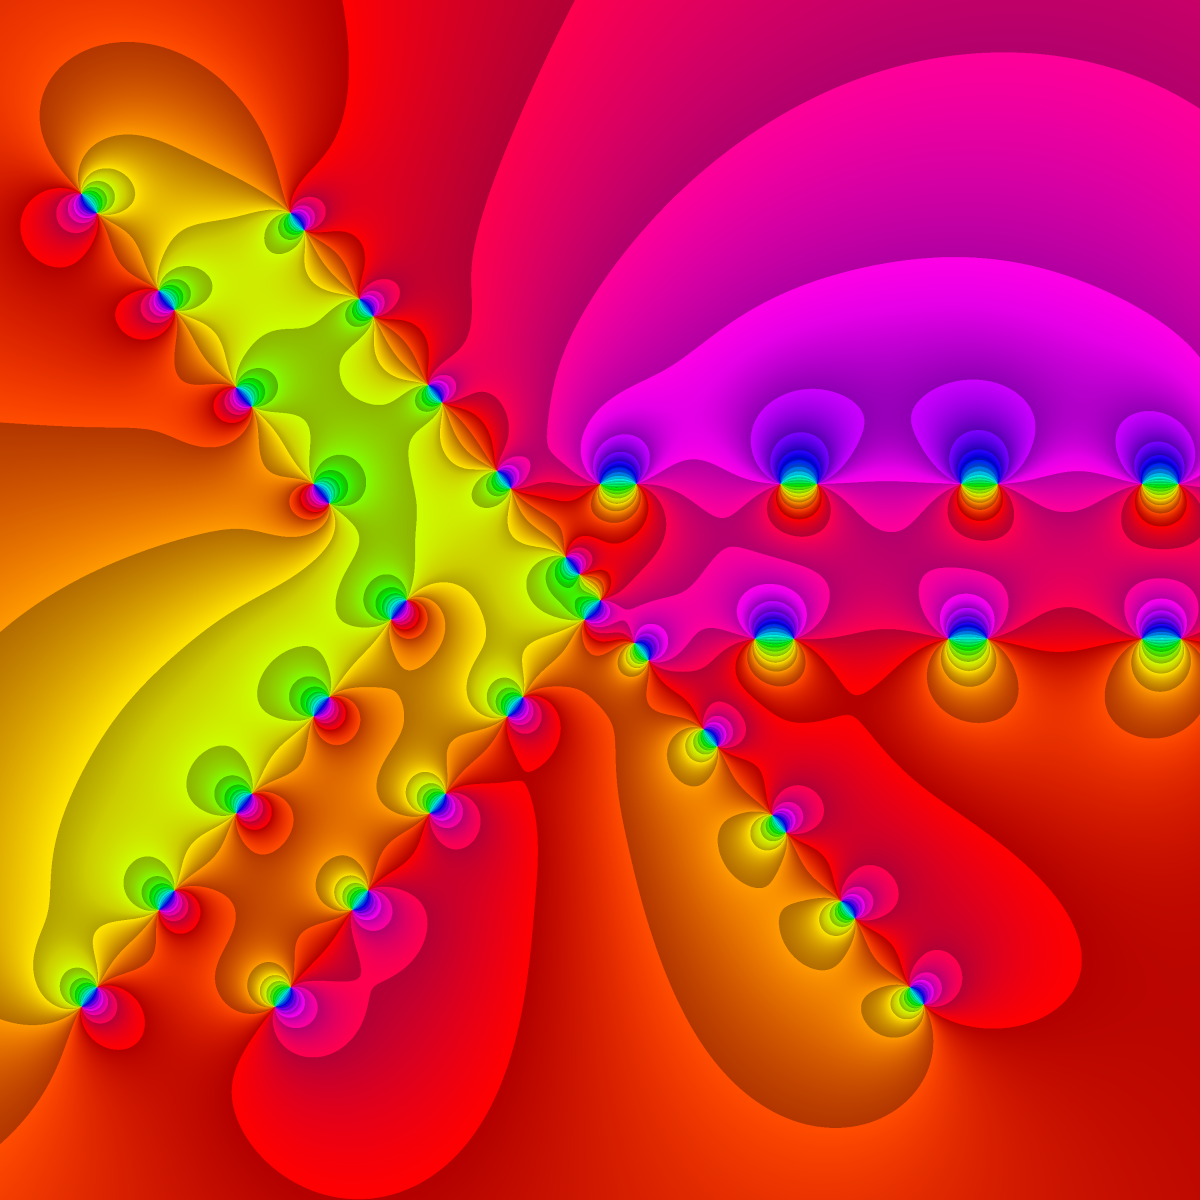
\includegraphics[width=\linewidth]{img/haskell_art}
  \caption{Art generation}
\end{subfigure}
~
\begin{subfigure}[t]{0.3\textwidth}
  \centering
  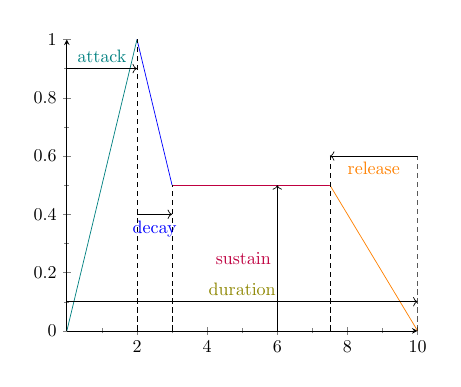
\begin{tikzpicture}[scale=0.65]
  \begin{axis}[
    minor tick num=1,
    samples=120,
    axis y line=left,
    axis x line=middle
    ]
    \addplot+[domain=0:10, mark=none, teal]
      coordinates {(0,0) (2, 1)};
    \addplot+[domain=0:10, mark=none, blue]
      coordinates {(2,1) (3, 0.5)};
    \addplot+[domain=0:10, mark=none, purple]
      coordinates {(3, 0.5) (7.5, 0.5)};
    \addplot+[domain=0:10, mark=none, orange]
      coordinates {(7.5, 0.5) (10, 0)};
    \addplot[densely dashed] coordinates {(2,0) (2,1)};
    \addplot[densely dashed] coordinates {(3,0) (3,0.5)};
    \addplot[densely dashed] coordinates {(7.5,0) (7.5,0.6)};
    \addplot[densely dashed] coordinates {(10,0) (10,0.6)};
    \addplot[->] coordinates {(0,0.9) (2,0.9)} node[midway, above, teal] {attack};
    \addplot[->] coordinates {(2,0.4) (3,0.4)} node[midway, below, blue] {decay};
    \addplot[->] coordinates {(6,0) (6,0.5)} node[midway,left, purple] {sustain};
    \addplot[<-] coordinates {(7.5,0.6) (10,0.6)} node[midway, below, orange] {release};
    \addplot[->] coordinates {(0,0.1) (10,0.1)} node[midway, above, olive] {duration};
  \end{axis}
  \end{tikzpicture}
  \caption{Music synthesis}
\end{subfigure}
\caption{Examples of exercises created as part of the course}
\end{figure*}

Many students at TUM have questioned the
applicability and usefulness
of functional languages after completing
the mandatory functional programming course.
We believe this is mainly due to two reasons:
\begin{enumerate*}[label=\arabic*)]
  \item introductory programming courses often stick
to simple algorithmic or mathematically inspired challenges and
\item side-effects (in particular I/O)
are often introduced very late
in functional programming courses.
\end{enumerate*}

Changing the latter appeared difficult to us:
we think that students would be confused
if a ``special'' \mintinline{Haskell}{IO} type and do notation were to
be introduced before they are comfortable
with the basic features of functional
languages.
We thus focused on the other issue
and created exercises that go beyond
simple terminal applications.
Designing and implementing such exercises,
however, is labour-intensive.
As mentioned in \cref{sec:engagement},
we thus decided to reallocate resources and
let our student assistants help us with this work
rather than providing feedback for homework submissions.

This turned out to be a very fruitful idea:
the quality of our student assistants' work was often way above what
we expected.
The one difficulty we faced was the mediocre quality of
tests written by most assistants
since they only had the rudimentary knowledge of QuickCheck taught as part of
the course.
We thus hosted a workshop for them that explained
our testing infrastructure and best-practice
patterns when writing tests.
The quality of tests significantly increased following this workshop,
though we still had to polish them before publication.

We next introduce a few exercises and tools
that were created as part of the course.
They are available in this article's repository\footnote{\url{https://github.com/kappelmann/engaging-large-scale-functional-programming}},
next to our other exercises, including
a music synthesiser framework,
a turtle graphics framework,
an UNO framework,
and guided exercises for DPLL and resolution provers.
Some further examples can be found on our competition blogs\footnote{\url{https://www21.in.tum.de/teaching/fpv/WS20/wettbewerb.html} (WS20) and
\url{https://www21.in.tum.de/teaching/fpv/WS19/wettbewerb.html} (WS19)}.

\paragraph{Game Tournament Framework}
It has become a course tradition to run a game tournament over the Christmas break.
In this tournament, the students are tasked with writing an AI for a board game that competes against the AIs of their fellow students.
To pass the homework sheet, it suffices to implement a basic strategy, but to score well in the competition, students came up with quite sophisticated strategies in past years.
The framework allows students to use statefulness and randomisation, so that there are few limits to the students' creativity.
The best strategies usually use the minimax rule with alpha-beta-pruning and a clever evaluation function, which is particularly important in this setting because the game tree cannot be evaluated very far given the time limit for each submission in the tournament.

The tournament runs continuously for 2--3 weeks and the results are displayed on a website (see \cref{fig:chainreaction} for an example from WS20).
Students thus get reasonably quick feedback on how their strategy performs,
which keeps them engaged and allows them to improve their strategy iteratively.
The tournament became a popular feature of the course with 182 participating students in WS19 and 220 in WS20.

In our repository, we provide the framework along with code specific to the game from WS20, which is based on Chain Reaction\footnote{\url{ https://brilliant.org/wiki/chain-reaction-game/}}.
It runs a round-robin tournament,
collecting statistics for each game and player.
Instructions for adapting the framework to a different game can also be found in the repository.

\paragraph{Programming Contest Framework}\label{sec:contest}
To foster social interaction and diversify the bonus system,
we hosted an ACM-ICPC-like programming contest.
In such contests, students
participate in teams of 2--3,
solving as many programming challenges as possible in a given time frame,
and can check their ranking on a live scoreboard.
% At some point during the contest,
% the scoreboard gets frozen,
% and following the working time,
% solutions to all challenges are presented by the organisers.
% The final results are then revealed by unfreezing the scoreboard again.

We found existing solutions
to run such contests too heavyweight for our purpose
and hence created a lightweight alternative.
Our framework continuously receives test results,
computes each team's score,
and displays the live scoreboard and task instructions.
It is agnostic to the programming language and test runner used.
It expects tests results adhering to the Apache Ant JUnit XML schema,
but modifying it to support other formats is straightforward.
Deployment instructions can be found in this article's repository.

We ran an online iteration of the contest in WS20,
again using ArTEMiS as a test runner.
Teams were cooperating on their platform of choice
and were able to ask for clarifications on a dedicated online channel.
Our experiences are very positive:
a total of 27 teams participated in the contest
and most stayed for the social hangout following it.
Given the presented framework,
the technical setup of the contest requires little time.
Some significant time, however,
must be spent on setting up the challenges,
tests, and solutions,
though plenty of challenges may be found
online by searching for other contests,
which one then may modify and reuse.
In general, we recommend running such contests
for every lecture concerned with programming concepts.

\section{I/O Mocking}
As discussed in Section~\ref{sec:tech_setup_test}, we primarily use QuickCheck to automatically assess submissions for homework exercises.
This brings up the question how monadic I/O in Haskell can be tested on the submission system as I/O is an important part of the lecture.
Since we don't want to actually realise the side effects that the code produces, the obvious solution is to use a mocked version of \mintinline{Haskell}{IO}.

A standard approach to mock \mintinline{Haskell}{IO}, which is put forward by packages such as \texttt{monad-mock}\footnote{\url{https://hackage.haskell.org/package/monad-mock}} and \texttt{HMock}\footnote{\url{https://hackage.haskell.org/package/HMock}}, is to first extract the side effects that are required for a certain computation into its own type class.
Then, since a type class naturally allows multiple implementations (instantiations) of those effects, we can provide an implementation that actually executes the side effects on the machine on the one hand; on the other hand, we can provide a version that just modifies a mocked version of the environment. 
To implement a function that copies a file, for example, we need two operations: one for reading a file and one for writing a file.
\begin{minted}{Haskell}
import qualified Prelude
import Prelude hiding (readFile, writeFile)

class Monad m => MonadFileSystem m where
  readFile :: FilePath -> m String
  writeFile :: FilePath -> String -> m ()
\end{minted}
The implementation is straightforward.
\begin{minted}{Haskell}
copyFile :: MonadFileSystem m => FilePath -> FilePath -> m ()
copyFile source target = do
  content <- readFile source
  writeFile target content
\end{minted}
Due to the definition of \mintinline{Haskell}{MonadFileSystem}, the instance for \mintinline{Haskell}{IO} is trivial. 
The mocked version can be implemented as a map from file names to file contents wrapped by the \mintinline{Haskell}{State} monad transformer to make it mutable.
We omit the instantiation of \mintinline{Haskell}{MonadFileSystem} for brevity.
Testing \mintinline{Haskell}{copyFile} is now as simple as checking whether the state of the file system is as expected after executing the function.
An example that includes the instance \mintinline{Haskell}{MonadFileSystem MockFileSystem} and a test can be found in the repository under \verb!resources/io_mocking/typeclass!.
\begin{minted}{Haskell}
instance MonadFileSystem IO where
  readFile = Prelude.readFile
  writeFile = Prelude.writeFile

data MockFileSystem = MockFileSystem (Map FilePath String)
instance MonadFileSystem (State MockFileSystem) where
  readFile = ...
  writeFile = ...
\end{minted}
While the above approach does the job for many use cases, it lacks one important property: transparency.
More specifically, the code of the students must contain or import \mintinline{Haskell}{MonadFileSystem} and the signatures of functions that use \mintinline{Haskell}{IO} must be adapted.
This is especially problematic because, as described in Section~\ref{sec:syllabus}, the lecture teaches \mintinline{Haskell}{IO} without mentioning monads, which are only introduced at the end of the lecture.

Instead of modifying the existing code, we bring in the mocking at a later phase, namely at the time of compilation.
We achieve this with a mixin that replaces the \mintinline{Haskell}{IO} module of the student submission with a mocked version where the mocked \mintinline{Haskell}{IO} type is realised in a similar way to the mock file system from above.
This time we aim for full transparency, though, so we not only need a file system but also handles such as standard input and output as well as the working directory.
All of those aspects of the machine state are summarised in the type \mintinline{Haskell}{RealWorld}.
Crucially, the type also contains a mock user represented by a computation of type \mintinline{Haskell}{IO ()} who is responsible for interacting with program of the student, that is, the user generates the input and reads the output.
For simplicity, we don't show the full type here.
As before, this type is wrapped by the \mintinline{Haskell}{State} monad transformer as well as two additional transformers \mintinline{Haskell}{PauseT} and \mintinline{Haskell}{ExceptT} in order to form the mocked \mintinline{Haskell}{IO} type.
\begin{minted}{Haskell}
data RealWorld = RealWorld {
  workDir :: FilePath,
  files :: Map File Text,
  handles :: Map Handle HandleData,
  user :: IO (),
  ...
}

newtype IO a =
  IO { unwrapIO :: ExceptT IOException (PauseT (State RealWorld)) a } 
\end{minted}
While the transformer \mintinline{Haskell}{ExceptT} simply adds I/O exceptions such as errors for insufficient permissions, the purpose of \mintinline{Haskell}{PauseT} is not obvious.
To understand its role, consider the following simple program that reads the user's name and greets them.
\begin{minted}{Haskell}
module Hello where

main = do
 name <- getLine
 putStrLn $ "Hello " ++ name
\end{minted}
In a normal (non-mocked) execution of the program, the program blocks and waits for input when \mintinline{Haskell}{getLine} is called.
Now, if our \mintinline{Haskell}{IO} type would only consist of a state monad, all the input to the program would need to be fixed in advance since the program can only be executed as a monolithic unit.
What we need instead is to suspend the program every time a blocking operation is called and transfer control over to our mock user.
The mock user then reacts to the output of the program and generates the input that the program is waiting for.
When the user is done, they, in turn, yield and the program of the student is resumed.

These considerations lead us to the monad below consisting of two operations: the first one pauses execution whereas the second one runs a computation of the monad until either \texttt{pause} is called or the computation finishes.
In the former case \mintinline{Haskell}{stepPauseT} returns a \mintinline{Haskell}{Left c} where \texttt{c} represents the rest of the computation; in other words, the part of the computation that is executed when resuming. 
Otherwise, the final result \texttt{r} of the computation is returned as \mintinline{Haskell}{Right r}.
It should be noted that the pause monad is an instance of the more general coroutine monad as provided by the \texttt{monad-coroutine}\footnote{\url{https://hackage.haskell.org/package/monad-coroutine}} package.
For the implementation details of the corresponding monad transformer \mintinline{Haskell}{PauseT} we refer to the repository.
\begin{minted}{Haskell}
class Monad m => MonadPause m where
  pause :: m ()
  stepPauseT :: m a -> m (Either (m a) a)
\end{minted}
We exemplify the mechanics of the mocking framework with simple test of the \texttt{main} method from above.
To this end, we first implement a mock user who, in our case, takes a name and supplies it to the standard input of \texttt{main}.
The user then reads the output of the program and checks whether it printed the expected greeting.
In the QuickCheck property \mintinline{Haskell}{prop_hello} we evaluate the interaction between the mock user and the program with \mintinline{Haskell}{Mock.evalIO} on \mintinline{Haskell}{Mock.emptyWorld}, a minimal \mintinline{Haskell}{RealWorld} that contains no files and only the absolutely necessary handles: standard input, standard output, and standard error.
The interaction itself sets the user to \texttt{user s}, then executes the \texttt{main} method, and finally runs the user to completion.
\begin{minted}{Haskell}
module Test where

import qualified Mock.System.IO.Internal as Mock
import qualified Hello as Sub

user :: String -> Mock.IO ()
user s = do
  Mock.hPutStrLn Mock.stdin s
  output <- Mock.hGetLine Mock.stdout
  when (output /= ("Hello " ++ s))
    (fail $ "\nExpected:\n" ++ "Hello " ++ s
      ++ "\nActual:\n" ++ output ++ "\n")

prop_hello = forAll (elements ["Karl", "Friedrich", "Rosa"]) $ \s ->
  Mock.evalIO (Mock.setUser (user s) >> Sub.main >> Mock.runUser)
              Mock.emptyWorld
\end{minted}
Figure~\ref{fig:iomocking} illustrates the steps that \mintinline{Haskell}{Mock.evalIO} takes while evaluating the interaction.
Note that there are two blocking operation, i.e.\ operations that call \texttt{pause} internally, namely \texttt{getLine} and \texttt{Mock.hGetLine Mock.stdout}.
When \mintinline{Haskell}{Mock.evalIO} encounters one of those it transfers control between the user and the program as indicated by the black arrows.
Of course, control is also transferred if the computation runs until completion without seeing a \texttt{pause}.
The horizontal axis with the white arrows illustrates the return values of \texttt{stepPauseT}. 
Focussing on the \mintinline{Haskell}{main} method, we see that, when encountering \texttt{getLine}, \texttt{stepPauseT} returns the remaining computation \mintinline{Haskell}{putStrLn $ "Hello " ++ x} wrapped in a \mintinline{Haskell}{Left}.
After the user provides the input for \texttt{getLine} and yields, the \mintinline{Haskell}{main} method prints the greeting and finishes with the result \mintinline{Haskell}{Right ()}.
Similarly, the user is blocked on \texttt{Mock.hGetLine} which means that the remaining computation only consists of the \texttt{when} check, which is executed as soon as \mintinline{Haskell}{main} is done.
This explains why we need to run \mintinline{Haskell}{Mock.runUser} after \mintinline{Haskell}{Sub.main} since the crucial \texttt{when} check would never be executed otherwise.

All in all, the mocking framework lets us uniformly test student submissions with the likes of QuickCheck and Smallcheck irregardless of whether they contain I/O programs.
\begin{figure}[h]
  \centering
\scalebox{0.75}{
\begin{tikzpicture}[cnode/.style={draw,rectangle,minimum height=2.5em}, >=stealth]
  \node[cnode] (P1) {\lstinputlisting[style=Haskell]{./sections/io_mocking/P.hs}};
  \node[cnode, right=2cm of P1.south east, anchor=south west] (P2) {\lstinputlisting[style=Haskell,firstline=2]{./sections/io_mocking/P.hs}};
  \node[cnode, right=2cm of P2.south east, anchor=south west] (P3) {\texttt{()}};

  \path (P1.south east) -- coordinate (MP12) (P2.south west);
  \path (P2.south east) -- coordinate (MP23) (P3.south west);
  \node[cnode, below=2cm of MP12, anchor=north] (U1) {\lstinputlisting[style=Haskell]{./sections/io_mocking/U.hs}};
  \node[cnode, below=2cm of MP23, anchor=north] (U2) {\lstinputlisting[style=Haskell,firstline=4]{./sections/io_mocking/U.hs}};
  \node[cnode, right=2cm of U2.north east, anchor=north west] (U3) {\texttt{()}};

  \path (U2.east |- U3) -- coordinate (MU23) (U3);
  \path (P3 -| MU23) -- node[shape=circle, fill=black, scale=0.8] (END) {} (MU23);

  \begin{scope}[>=open triangle 45]
    \draw[->] (P1.east |- P2) -- node[above] {\texttt{Left}} (P2);
    \draw[->] (P2.east |- P3) -- node[above] {\texttt{Right}} (P3);
    \draw[->] (U1.east |- U2) -- node[below] {\texttt{Left}} (U2);
    \draw[->] (U2.east |- U3) -- node[below] {\texttt{Right}} (U3);
  \end{scope}

  \begin{scope}[>=triangle 45]
    \draw[->] (P1.east |- P2) to[out=0, in=90] (U1);
    \draw[->] (P2.east |- P3) to[out=0, in=90] (U2);
    \draw[->] (U1.east |- U2) to[out=0, in=-90, looseness=0.85] (P2);
    \draw[->] (U2.east |- U3) to[out=0, in=-90] (END);
  \end{scope}

\end{tikzpicture}
}
\caption{
  Interaction between the mock user and the student's submission.
  White arrows indicate the return value of \texttt{stepPauseT} whereas black arrows indicate transfer of control.
  The black dot signifies the end of the interaction.\label{fig:iomocking}
}
\end{figure}





\section{I/O Mocking}
As discussed in Section~\ref{sec:tech_setup_test}, we primarily use QuickCheck to automatically assess submissions for homework exercises.
This brings up the question how monadic I/O in Haskell can be tested on the submission system as I/O is an important part of the lecture.
Since we don't want to actually realise the side effects that the code produces, the obvious solution is to use a mocked version of \mintinline{Haskell}{IO}.

A standard approach to mock \mintinline{Haskell}{IO}, which is put forward by packages such as \texttt{monad-mock}\footnote{\url{https://hackage.haskell.org/package/monad-mock}} and \texttt{HMock}\footnote{\url{https://hackage.haskell.org/package/HMock}}, is to first extract the side effects that are required for a certain computation into its own type class.
Then, since a type class naturally allows multiple implementations (instantiations) of those effects, we can provide an implementation that actually executes the side effects on the machine on the one hand; on the other hand, we can provide a version that just modifies a mocked version of the environment. 
To implement a function that copies a file, for example, we need two operations: one for reading a file and one for writing a file.
\begin{minted}{Haskell}
import qualified Prelude
import Prelude hiding (readFile, writeFile)

class Monad m => MonadFileSystem m where
  readFile :: FilePath -> m String
  writeFile :: FilePath -> String -> m ()
\end{minted}
The implementation is straightforward.
\begin{minted}{Haskell}
copyFile :: MonadFileSystem m => FilePath -> FilePath -> m ()
copyFile source target = do
  content <- readFile source
  writeFile target content
\end{minted}
Due to the definition of \mintinline{Haskell}{MonadFileSystem}, the instance for \mintinline{Haskell}{IO} is trivial. 
The mocked version can be implemented as a map from file names to file contents wrapped by the \mintinline{Haskell}{State} monad transformer to make it mutable.
We omit the instantiation of \mintinline{Haskell}{MonadFileSystem} for brevity.
Testing \mintinline{Haskell}{copyFile} is now as simple as checking whether the state of the file system is as expected after executing the function.
An example that includes the instance \mintinline{Haskell}{MonadFileSystem MockFileSystem} and a test can be found in the repository under \verb!resources/io_mocking/typeclass!.
\begin{minted}{Haskell}
instance MonadFileSystem IO where
  readFile = Prelude.readFile
  writeFile = Prelude.writeFile

data MockFileSystem = MockFileSystem (Map FilePath String)
instance MonadFileSystem (State MockFileSystem) where
  readFile = ...
  writeFile = ...
\end{minted}
While the above approach does the job for many use cases, it lacks one important property: transparency.
More specifically, the code of the students must contain or import \mintinline{Haskell}{MonadFileSystem} and the signatures of functions that use \mintinline{Haskell}{IO} must be adapted.
This is especially problematic because, as described in Section~\ref{sec:syllabus}, the lecture teaches \mintinline{Haskell}{IO} without mentioning monads, which are only introduced at the end of the lecture.

Instead of modifying the existing code, we bring in the mocking at a later phase, namely at the time of compilation.
We achieve this with a mixin that replaces the \mintinline{Haskell}{IO} module of the student submission with a mocked version where the mocked \mintinline{Haskell}{IO} type is realised in a similar way to the mock file system from above.
This time we aim for full transparency, though, so we not only need a file system but also handles such as standard input and output as well as the working directory.
All of those aspects of the machine state are summarised in the type \mintinline{Haskell}{RealWorld}.
Crucially, the type also contains a mock user represented by a computation of type \mintinline{Haskell}{IO ()} who is responsible for interacting with program of the student, that is, the user generates the input and reads the output.
For simplicity, we don't show the full type here.
As before, this type is wrapped by the \mintinline{Haskell}{State} monad transformer as well as two additional transformers \mintinline{Haskell}{PauseT} and \mintinline{Haskell}{ExceptT} in order to form the mocked \mintinline{Haskell}{IO} type.
\begin{minted}{Haskell}
data RealWorld = RealWorld {
  workDir :: FilePath,
  files :: Map File Text,
  handles :: Map Handle HandleData,
  user :: IO (),
  ...
}

newtype IO a =
  IO { unwrapIO :: ExceptT IOException (PauseT (State RealWorld)) a } 
\end{minted}
While the transformer \mintinline{Haskell}{ExceptT} simply adds I/O exceptions such as errors for insufficient permissions, the purpose of \mintinline{Haskell}{PauseT} is not obvious.
To understand its role, consider the following simple program that reads the user's name and greets them.
\begin{minted}{Haskell}
module Hello where

main = do
 name <- getLine
 putStrLn $ "Hello " ++ name
\end{minted}
In a normal (non-mocked) execution of the program, the program blocks and waits for input when \mintinline{Haskell}{getLine} is called.
Now, if our \mintinline{Haskell}{IO} type would only consist of a state monad, all the input to the program would need to be fixed in advance since the program can only be executed as a monolithic unit.
What we need instead is to suspend the program every time a blocking operation is called and transfer control over to our mock user.
The mock user then reacts to the output of the program and generates the input that the program is waiting for.
When the user is done, they, in turn, yield and the program of the student is resumed.

These considerations lead us to the monad below consisting of two operations: the first one pauses execution whereas the second one runs a computation of the monad until either \texttt{pause} is called or the computation finishes.
In the former case \mintinline{Haskell}{stepPauseT} returns a \mintinline{Haskell}{Left c} where \texttt{c} represents the rest of the computation; in other words, the part of the computation that is executed when resuming. 
Otherwise, the final result \texttt{r} of the computation is returned as \mintinline{Haskell}{Right r}.
It should be noted that the pause monad is an instance of the more general coroutine monad as provided by the \texttt{monad-coroutine}\footnote{\url{https://hackage.haskell.org/package/monad-coroutine}} package.
For the implementation details of the corresponding monad transformer \mintinline{Haskell}{PauseT} we refer to the repository.
\begin{minted}{Haskell}
class Monad m => MonadPause m where
  pause :: m ()
  stepPauseT :: m a -> m (Either (m a) a)
\end{minted}
We exemplify the mechanics of the mocking framework with simple test of the \texttt{main} method from above.
To this end, we first implement a mock user who, in our case, takes a name and supplies it to the standard input of \texttt{main}.
The user then reads the output of the program and checks whether it printed the expected greeting.
In the QuickCheck property \mintinline{Haskell}{prop_hello} we evaluate the interaction between the mock user and the program with \mintinline{Haskell}{Mock.evalIO} on \mintinline{Haskell}{Mock.emptyWorld}, a minimal \mintinline{Haskell}{RealWorld} that contains no files and only the absolutely necessary handles: standard input, standard output, and standard error.
The interaction itself sets the user to \texttt{user s}, then executes the \texttt{main} method, and finally runs the user to completion.
\begin{minted}{Haskell}
module Test where

import qualified Mock.System.IO.Internal as Mock
import qualified Hello as Sub

user :: String -> Mock.IO ()
user s = do
  Mock.hPutStrLn Mock.stdin s
  output <- Mock.hGetLine Mock.stdout
  when (output /= ("Hello " ++ s))
    (fail $ "\nExpected:\n" ++ "Hello " ++ s
      ++ "\nActual:\n" ++ output ++ "\n")

prop_hello = forAll (elements ["Karl", "Friedrich", "Rosa"]) $ \s ->
  Mock.evalIO (Mock.setUser (user s) >> Sub.main >> Mock.runUser)
              Mock.emptyWorld
\end{minted}
Figure~\ref{fig:iomocking} illustrates the steps that \mintinline{Haskell}{Mock.evalIO} takes while evaluating the interaction.
Note that there are two blocking operation, i.e.\ operations that call \texttt{pause} internally, namely \texttt{getLine} and \texttt{Mock.hGetLine Mock.stdout}.
When \mintinline{Haskell}{Mock.evalIO} encounters one of those it transfers control between the user and the program as indicated by the black arrows.
Of course, control is also transferred if the computation runs until completion without seeing a \texttt{pause}.
The horizontal axis with the white arrows illustrates the return values of \texttt{stepPauseT}. 
Focussing on the \mintinline{Haskell}{main} method, we see that, when encountering \texttt{getLine}, \texttt{stepPauseT} returns the remaining computation \mintinline{Haskell}{putStrLn $ "Hello " ++ x} wrapped in a \mintinline{Haskell}{Left}.
After the user provides the input for \texttt{getLine} and yields, the \mintinline{Haskell}{main} method prints the greeting and finishes with the result \mintinline{Haskell}{Right ()}.
Similarly, the user is blocked on \texttt{Mock.hGetLine} which means that the remaining computation only consists of the \texttt{when} check, which is executed as soon as \mintinline{Haskell}{main} is done.
This explains why we need to run \mintinline{Haskell}{Mock.runUser} after \mintinline{Haskell}{Sub.main} since the crucial \texttt{when} check would never be executed otherwise.

All in all, the mocking framework lets us uniformly test student submissions with the likes of QuickCheck and Smallcheck irregardless of whether they contain I/O programs.
\begin{figure}[h]
  \centering
\scalebox{0.75}{
\begin{tikzpicture}[cnode/.style={draw,rectangle,minimum height=2.5em}, >=stealth]
  \node[cnode] (P1) {\lstinputlisting[style=Haskell]{./sections/io_mocking/P.hs}};
  \node[cnode, right=2cm of P1.south east, anchor=south west] (P2) {\lstinputlisting[style=Haskell,firstline=2]{./sections/io_mocking/P.hs}};
  \node[cnode, right=2cm of P2.south east, anchor=south west] (P3) {\texttt{()}};

  \path (P1.south east) -- coordinate (MP12) (P2.south west);
  \path (P2.south east) -- coordinate (MP23) (P3.south west);
  \node[cnode, below=2cm of MP12, anchor=north] (U1) {\lstinputlisting[style=Haskell]{./sections/io_mocking/U.hs}};
  \node[cnode, below=2cm of MP23, anchor=north] (U2) {\lstinputlisting[style=Haskell,firstline=4]{./sections/io_mocking/U.hs}};
  \node[cnode, right=2cm of U2.north east, anchor=north west] (U3) {\texttt{()}};

  \path (U2.east |- U3) -- coordinate (MU23) (U3);
  \path (P3 -| MU23) -- node[shape=circle, fill=black, scale=0.8] (END) {} (MU23);

  \begin{scope}[>=open triangle 45]
    \draw[->] (P1.east |- P2) -- node[above] {\texttt{Left}} (P2);
    \draw[->] (P2.east |- P3) -- node[above] {\texttt{Right}} (P3);
    \draw[->] (U1.east |- U2) -- node[below] {\texttt{Left}} (U2);
    \draw[->] (U2.east |- U3) -- node[below] {\texttt{Right}} (U3);
  \end{scope}

  \begin{scope}[>=triangle 45]
    \draw[->] (P1.east |- P2) to[out=0, in=90] (U1);
    \draw[->] (P2.east |- P3) to[out=0, in=90] (U2);
    \draw[->] (U1.east |- U2) to[out=0, in=-90, looseness=0.85] (P2);
    \draw[->] (U2.east |- U3) to[out=0, in=-90] (END);
  \end{scope}

\end{tikzpicture}
}
\caption{
  Interaction between the mock user and the student's submission.
  White arrows indicate the return value of \texttt{stepPauseT} whereas black arrows indicate transfer of control.
  The black dot signifies the end of the interaction.\label{fig:iomocking}
}
\end{figure}

\section{Check Your Proof by Example}\label{sec:cyp}
In addition to functional programming, the course we taught is also concerned with verification of programs; more specifically functional programs.
Even if we only consider a small total subset of Haskell, equational reasoning together with induction (and case analysis) is already sufficient to prove interesting properties.
Since fast and loose reasoning is morally correct~\cite{fast_and_loose}, valid properties in this sub-language are also valid for Haskell.
Simple inductive proofs of course lend themselves well to be automatically checked and, as announced by \cite{next_1100}, a tool called ``Check Your Proof'' (CYP for short) was developed at our lab by Durner and Noschinski\footnote{\url{https://github.com/noschinl/cyp}}.
The first example of an inductive proof in the lecture is the associativity of append on lists.
Transferring this example to CYP requires us to define the data type of lists.
We use \lstinline![]! as the constructor of the empty list and the infix operator \lstinline!:! like in Haskell.
\begin{lstlisting}
data List a = [] | a : List a
\end{lstlisting}
Now we can define append as the customary infix operator \lstinline!++! and state the goal \lstinline!xs ++ (ys ++ zs) .=. (xs ++ ys) ++ zs! where all variables are implicitly universally quantified.
\begin{lstlisting}
[] ++ ys = ys
(x : xs) ++ ys = x : (xs ++ ys)
goal xs ++ (ys ++ zs) .=. (xs ++ ys) ++ zs
\end{lstlisting}
The listings above make up the background theory for this particular proof.
These definitions are meant to be provided to the students by the instructors and are not to be modified.
The students then supply the proof in a separate file.
In our case, we proceed to prove the statement by structural induction on \lstinline!xs!.
\begin{lstlisting}
Lemma: xs ++ (ys ++ zs) .=. (xs ++ ys) ++ zs
Proof by induction on List xs
  Case []
    To show: [] ++ (ys ++ zs) .=. ([] ++ ys) ++ zs
    Proof
                      [] ++ (ys ++ zs)
      (by def ++) .=. ys ++ zs
      (by def ++) .=. ([] ++ ys) ++ zs
    QED
\end{lstlisting}
In the listing above, the first \lstinline!Proof! marks the beginning of an inductive proof whereas the second \lstinline!Proof!, which has no further arguments, starts an equational proof.
While CYP allows arbitrary nesting of proofs by case analysis or induction, at the innermost level it always is down to an equational proof to discharge the goal.
An equational proof is a chain of equalities that rewrite the left-hand side of the current goal to the right-hand side.
Note that in the example \lstinline!(by def ++)! refers to either one of the defining equations of \lstinline!++! so CYP will try if any of them justifies the current step.
The user has to justify each rewrite step by a corresponding equation that, when applied to the term or a subterm on the left-hand side, yields the right-hand side.

Now, consider the inductive case.
\begin{lstlisting}
  Case x : xs
    To show: (x : xs) ++ (ys ++ zs) .=. ((x : xs) ++ ys) ++ zs
    IH: xs ++ (ys ++ zs) .=. (xs ++ ys) ++ zs
    Proof
                        (x : xs) ++ (ys ++ zs)
      (by def ++)   .=. x : (xs ++ (ys ++ zs))
      (by IH)       .=. x : ((xs ++ ys) ++ zs)
      (by def ++)   .=. (x : (xs ++ ys)) ++ zs
      (by def ++)   .=. ((x : xs) ++ ys) ++ zs
    QED
QED
\end{lstlisting}
Again, CYP requires the user to be explicit: the goal in each inductive case and the induction hypotheses have to be spelled out.

The lecture then goes beyond proofs by structural induction and introduces proof by extensionality, case analysis, and computation induction, all of which CYP supports with some conditions applying as we will see shortly.
Computation induction in particular was not supported in the original version by Durner and Noschinski but was only introduced in a fork\footnote{\url{https://github.com/lukasstevens/cyp}}.
Furthermore, CYP allows proving named lemmas to modularise proofs and to prove generalised versions of the goal, which is for example necessary to show certain properties of \lstinline!fold!.

The simplicity of CYP both in its usage and its implementation brings with it some caveats:
\begin{itemize}
    \item The version of CYP that we use is untyped and thus unsound if the background theory contains multiple types as \cite{cyp_holes} demonstrate: if you have a singleton type \lstinline!data U = U! in your background theory, you can prove \lstinline!x .=. y! by case analysis.
        In an untyped environment you can then use this to prove equality between any two terms.
    \item Barring soundness issues due to a lack of types, one also needs to ensure that all function definitions are total and that their patterns do not overlap.
    \item Computation induction is only sound if there are no recursive calls in branches of an if-then-else expression.
      This is because the induction hypotheses then would need to be conditional rewrite rules which CYP does not support.
\end{itemize}
\cite{cyp_holes} discuss the inner workings of CYP in detail and develop an extension to CYP that introduces types thus solving the first issue.
In the process they also made it possible to leave holes in proofs and in expressions for the students to fill in, which makes it a more flexible tool for teaching.
Solving the latter issues would incur additional effort.
We think that CYP should be put on a stronger foundation such as higher-order logic (HOL) without compromising its simplicity from a user perspective.
One possibility would be to rewrite CYP as as a frontend to Isabelle/HOL~\cite{isabelle}.
Since HOL is a typed logic it would solve the first issue and the latter issues could be resolved using Isabelle's function package~\cite{isabelle_functions}.
A stronger foundation also allows one to more confidently develop further extensions to CYP.

Our experience with using CYP to teach inductive proofs have been very positive.
On the one hand, CYP is scalable since it has an integration with the same testing framework, Tasty\footnote{\url{https://hackage.haskell.org/package/tasty}}, that is used to mark programming exercises automatically.
This allows us to deal with programming and proof exercises in a uniform way.
On the other hand, CYP was engaging to the students as their feedback shows:
in the first iteration of the lecture, we received two positive comments and one negative comment without asking for feedback on CYP.
When asked explicitly about their thoughts on CYP the second time around, the students answered with 18 positive comments and three negative comments.
The students liked the instantaneous feedback that CYP provides, which helped them to deepen their understanding of inductive proofs at their own pace.
The main criticism of CYP was the lack of documentation.
A cheatsheet developed by a tutor was later added to the repository of CYP to improve the situation.

\lukas{Move this to exam section? Also mention that uniform structure makes it easier to grade}
In each of the exams, two exercises (out of 7 -- 9) were concerned with inductive proofs.
The first exercise was a straightforward proof by structural induction while the second exercise required more creativity, e.g.\ generalisation of the goal or a computational induction.
We did not force the students to stick to CYP's syntax in the exam but we urged them to follow a similar structure, which worked well overall.

% Teaching experiences
% \begin{itemize}
%     \item Should use non-standard data types in the exam since some students just copy the induction schema otherwise.
%     \item Student feedback mostly positive as in the other paper.
%     \item Students write well structured proofs in the exam that resemble cyp proofs.
%     \item VSCode/vim highlighting thanks to students, tutors.
%     \item Proofs can automatically be checked by the submission system.
% \end{itemize}
%
% \begin{itemize}
%   \item Why cyp? Maybe ask Lars Noschinski about cyp
%   \item \href{https://arxiv.org/pdf/2009.01326.pdf}{Other CYP Paper}. Why is this only in the pre-proceedings of WFLP 2020?
%   \item Kind of exercises throughout the course.
%   \item 2020: on two tutorial sheets (3 exercises), Tutorial 4: 1, Homework 4: 2, Tutorial 5: 2, Homework 5: 1, Tutorial 9: 1, Homework 9: 1, Tutorial 13: 1, Exam: 2(Structural, Structural + Aux Lemma)/9, Retake: 2(Structural, Computation)/7
%   \item 2019: Exam 2(Structural, Structural + Generalisation)/8, Retake: 2(Structural, Computation)/7, Tutorial 5: 2, Homework 5: 2, Tutorial 6: 2, Homework 6: 2, Tutorial 7: 1, Homework 7: 1, Tutorial 9: 1, Homework 9: 1, Tutorial 13: 1
%   \item 2019 Retake has computation induction but no CYP. Maybe compare results?
%   \item 2019 CYP Feedback: positiv 2, negativ 1
%   \item 2020 CYP Feedback: positiv 18, negativ 3 (Mainly documentation)
%   \item Uses haskell-src-exts for parsing Haskell code
% \end{itemize}

\section{Exams}\label{sec:exam}
In previous iterations of the course, the exams had been paper-based by necessity, as university regulations made digital exams unfeasible. Due to the COVID-19 pandemic, however, remote exams (either unsupervised or supervised via video conferencing software) were allowed for the repeat exam in WS19 and both exams in WS20.

In the following we will outline how we adapted our exam process to this new reality and the advantages of our approach for students and staff.

\paragraph{Workflow for Students}

We chose the ArTEMiS \citep{artemis} platform, previously described in \cref{sec:tech_setup_test}, for the exams. In WS19, the students were previously mostly unfamiliar with ArTEMiS, but in WS20 they had been submitting their homeworks using the same workflow as during the exam.

Students were able to check out individual exam questions from the ArTEMiS repository and then work on them using their preferred programming environment. In addition to programming exercises, the exams included theory questions and proofs, which were submitted as text using an online editor.

The exams were open-book, including online resources. We feel that the combination of a programming environment customized to the individual student's taste and access to online documentation, forums, etc.~comes close to how programming is done in practice. \jonas{Numbers for value of standardized environment?}

In contrast, previous exams were purely paper-based. This limited the scope of programming exercises we were able to pose, since both writing and grading programs on paper is highly labor intensive. In addition, we were able to expect a higher standard of correctness from the submitted programs,

\paragraph{Grading}
Grading hundreds of exams on paper is a huge undertaking. In previous semesters, it took 10-20 people (staff and student assistants) about 4-5 days \jonas{actual numbers from endterm 19} to grade an exam. Additionally, grading programming exercises on paper is error prone, as it is not feasible to digitize every submission and run it through a compiler.

Using ArtEMiS, we were able to use automated testing for programming exercises. In most cases we were able to mark submissions which passed all tests as fully correct and manual grading was only needed for submissions which failed some tests or did not compile. This significantly lightened the workload, as even manual grading is much more convenient when there are test results to guide you and when you can re-run tests after fixing compilation errors.

In addition, the feedback for the students is vastly improved by this method of grading, since they are able to check test results in the exam review instead of having to rely on handwritten annotations made by the corrector.

\jonas{how much person hours to correct endterm 20?}

\paragraph{Cheating}

\jonas{anecdotal evidence of little cheating/plagiarism. just leave this out entirely?}

\section{Conclusion}\label{sec:conclusion}

TODO


\bibliographystyle{eptcs}
\bibliography{sources}
\end{document}

